\documentclass{beamer}
\mode<presentation>
\usepackage{amsmath}
\usepackage{amssymb}
%\usepackage{advdate}
\usepackage{adjustbox}
\usepackage{subcaption}
\usepackage{enumitem}
\usepackage{multicol}
\usepackage{gensymb}
\usepackage{mathtools}
\usepackage{listings}
\usepackage{url}
\def\UrlBreaks{\do\/\do-}
\usetheme{Boadilla}
\usecolortheme{lily}
\setbeamertemplate{footline}
{
  \leavevmode%
  \hbox{%
  \begin{beamercolorbox}[wd=\paperwidth,ht=2ex,dp=1ex,right]{author in head/foot}%
    \insertframenumber{} / \inserttotalframenumber\hspace*{2ex} 
  \end{beamercolorbox}}%
  \vskip0pt%
}
\setbeamertemplate{navigation symbols}{}

\providecommand{\nCr}[2]{\,^{#1}C_{#2}} % nCr
\providecommand{\nPr}[2]{\,^{#1}P_{#2}} % nPr
\providecommand{\mbf}{\mathbf}
\providecommand{\pr}[1]{\ensuremath{\Pr\left(#1\right)}}
\providecommand{\qfunc}[1]{\ensuremath{Q\left(#1\right)}}
\providecommand{\sbrak}[1]{\ensuremath{{}\left[#1\right]}}
\providecommand{\lsbrak}[1]{\ensuremath{{}\left[#1\right.}}
\providecommand{\rsbrak}[1]{\ensuremath{{}\left.#1\right]}}
\providecommand{\brak}[1]{\ensuremath{\left(#1\right)}}
\providecommand{\lbrak}[1]{\ensuremath{\left(#1\right.}}
\providecommand{\rbrak}[1]{\ensuremath{\left.#1\right)}}
\providecommand{\cbrak}[1]{\ensuremath{\left\{#1\right\}}}
\providecommand{\lcbrak}[1]{\ensuremath{\left\{#1\right.}}
\providecommand{\rcbrak}[1]{\ensuremath{\left.#1\right\}}}
\theoremstyle{remark}
\newtheorem{rem}{Remark}
\newcommand{\sgn}{\mathop{\mathrm{sgn}}}
\providecommand{\abs}[1]{\left\vert#1\right\vert}
\providecommand{\res}[1]{\Res\displaylimits_{#1}} 
\providecommand{\norm}[1]{\lVert#1\rVert}
\providecommand{\mtx}[1]{\mathbf{#1}}
\providecommand{\mean}[1]{E\left[ #1 \right]}
\providecommand{\fourier}{\overset{\mathcal{F}}{ \rightleftharpoons}}
%\providecommand{\hilbert}{\overset{\mathcal{H}}{ \rightleftharpoons}}
\providecommand{\system}{\overset{\mathcal{H}}{ \longleftrightarrow}}
	%\newcommand{\solution}[2]{\textbf{Solution:}{#1}}
%\newcommand{\solution}{\noindent \textbf{Solution: }}
\providecommand{\dec}[2]{\ensuremath{\overset{#1}{\underset{#2}{\gtrless}}}}
\newcommand{\myvec}[1]{\ensuremath{\begin{pmatrix}#1\end{pmatrix}}}
\let\vec\mathbf

\lstset{
%language=C,
frame=single, 
breaklines=true,
columns=fullflexible
}

\numberwithin{equation}{section}

\title{Matgeo Presentation}
\author{G. Abhimanyu Koushik \\ EE24BTECH11024}

\date{\today} 
\begin{document}

\begin{frame}
\titlepage
\end{frame}

\section*{Outline}
\begin{frame}
\tableofcontents
\end{frame}
\section{Problem}
\begin{frame}
\frametitle{Problem Statement}
%
Construct a Triangle $ABC$ such that $\angle B=60\degree$, $\angle C=45\degree$ and $AB+BC+CA=12cm$.
%
\end{frame}

%\subsection{Literature}
\section{Solution}
\subsection{Input Parameters}
\begin{frame}
\frametitle{Input Parameters}
%\framesubtitle{Literature}
\begin{table}[H]    
  \centering
  \begin{tabular}[12pt]{ |c|c|c|}
    \hline
    \textbf{Symbol} & \textbf{Value} & \textbf{Description} \\
    \hline
    $\vec{A}$ & \myvec{6\\5} & First point\\
    \hline 
    $\vec{B}$ & \myvec{-4\\3} & Second point\\
    \hline
    $\vec{Y}$ & \myvec{0\\$y$} & Point on Y-Axis equidistant from A and B\\
    \hline
    \end{tabular}

\end{table}
\end{frame}
\subsection{Linear Equation}
\begin{frame}
\frametitle{Linear Equation}
%\framesubtitle{Literature}
From properties of triangle we get the following equations
%
\begin{align}
a+b+c&=K\\
b\cos(C)+c\cos(B)&=a\\
\frac{b}{\sin(B)}&=\frac{c}{\sin(C)}
\end{align}
%
\end{frame}
\subsection{Matrix Equation}
\begin{frame}
\frametitle{Matrix Equation}
The linear equations can be expxressed as
%\begin{enumerate}[label=(\roman*)]
\begin{align}
a+b+c&=K\\
-a+b\cos(C)+c\cos(B)&=0\\
b\sin(C)-c\sin(B)&=0
\end{align}
%
resulting in the matrix equation
\begin{align}
\label{eq:equation}
  \frac{1}{K}\myvec{1 & 1 & 1\\-1 & \cos{C} & \cos{B}\\0 & \sin{C} & -\sin{B}}\times\vec{x}&=\myvec{1\\0\\0}
\end{align}
where
\begin{align}
\vec{x} &= \myvec{a\\b\\c}
\end{align}
\end{frame}


\subsection{Row Reduction}
\begin{frame}
\frametitle{Row Reduction}
After substituting the values, \eqref{eq:equation} can be row reduced as follows
%
\begin{align}
\label{eq:mat_row}
\myvec{1 & 1 & 1 & 1\\-1 & \frac{1}{\sqrt{2}} & \frac{1}{2} & 0\\0 & \frac{1}{\sqrt{2}} & -\frac{\sqrt{3}}{2} & 0} \xleftrightarrow[]{R_2 \leftarrow {R_1+R_2}}\myvec{1 & 1 & 1 & 1\\0 & \frac{1}{\sqrt{2}}+1 & \frac{3}{2} & 1\\0 & \frac{1}{\sqrt{2}} & -\frac{\sqrt{3}}{2} & 0}\\
  \xleftrightarrow[]{R_3 \leftarrow {R_2-\brak{\sqrt{2}+1}R_3}}\myvec{1 & 1 & 1 & 1\\0 & \frac{1}{\sqrt{2}}+1 & \frac{3}{2} & 1\\0 & 0 & \brak{\sqrt{3}+\sqrt{2}+1}\frac{\sqrt{3}}{2} & 1}\\
  \xleftrightarrow[]{R_3 \leftarrow {\brak{\frac{2}{\sqrt{3}\brak{\sqrt{3}+\sqrt{2}+1}}}R_3}}\myvec{1 & 1 & 1 & 1\\0 & \frac{1}{\sqrt{2}}+1 & \frac{3}{2} & 1\\0 & 0 & 1 & \frac{2}{\sqrt{3}\brak{\sqrt{3}+\sqrt{2}+1}}}\\
  \xleftrightarrow[]{R_2 \leftarrow {R_2-\brak{\frac{3}{2}}R_3}}\myvec{1 & 1 & 1 & 1\\0 & \frac{1}{\sqrt{2}}+1 & 0 & \frac{\sqrt{2}+1}{\sqrt{3}+\sqrt{2}+1}\\0 & 0 & 1 & \frac{2}{\sqrt{3}\brak{\sqrt{3}+\sqrt{2}+1}}}
 \end{align}
\end{frame}
\begin{frame}
 \begin{align}
  \xleftrightarrow[]{R_2 \leftarrow \brak{\frac{\sqrt{2}}{\sqrt{2}+1}}R_2}\myvec{1 & 1 & 1 & 1\\0 & 1 & 0 & \frac{\sqrt{2}}{\sqrt{3}+\sqrt{2}+1}\\0 & 0 & 1 & \frac{2}{\sqrt{3}\brak{\sqrt{3}+\sqrt{2}+1}}}\\
  \xleftrightarrow[]{R_1 \leftarrow R_1-R_2}\myvec{1 & 0 & 1 & \frac{\sqrt{3}+1}{\sqrt{3}+\sqrt{2}+1}\\0 & 1 & 0 & \frac{\sqrt{2}}{\sqrt{3}+\sqrt{2}+1}\\0 & 0 & 1 & \frac{2}{\sqrt{3}\brak{\sqrt{3}+\sqrt{2}+1}}}\\
  \xleftrightarrow[]{R_1 \leftarrow R_1-R_3}\myvec{1 & 0 & 0 & \frac{1+\sqrt{3}}{\sqrt{3}\brak{\sqrt{3}+\sqrt{2}+1}}\\0 & 1 & 0 & \frac{1+\sqrt{3}}{\sqrt{3}\brak{\sqrt{3}+\sqrt{2}+1}}\\0 & 0 & 1 & \frac{2}{\sqrt{3}\brak{\sqrt{3}+\sqrt{2}+1}}}
\end{align}
\end{frame}
%\section{Plot}
\subsection{Final Answer}
\begin{frame}[fragile]
\frametitle{Final Answer}

Thus, 
\begin{align}
\label{eq:solution}
\brak{\frac{1}{K}}\vec{x}&=\myvec{\frac{1+\sqrt{3}}{\sqrt{3}\brak{\sqrt{3}+\sqrt{2}+1}}\\\frac{1+\sqrt{3}}{\sqrt{3}\brak{\sqrt{3}+\sqrt{2}+1}}\\\frac{2}{\sqrt{3}\brak{\sqrt{3}+\sqrt{2}+1}}}
\\
\implies a&=\frac{12+12\sqrt{3}}{\sqrt{3}\brak{\sqrt{3}+\sqrt{2}+1}}\\
b&=\frac{12\sqrt{2}}{\brak{\sqrt{3}+\sqrt{2}+1}}\\
c&=\frac{24}{\sqrt{3}\brak{\sqrt{3}+\sqrt{2}+1}}
\end{align}
%
The codes below verifies \eqref{eq:solution}.
\end{frame}

\section{C Code}
\begin{frame}[fragile]
\frametitle{C Code}
\begin{lstlisting}[language=C]
#include <stdio.h>
#include <stdlib.h>
#include <string.h>
#include <math.h>
#include <unistd.h>
#include "libs/matfun.h"
#include "libs/geofun.h"

void point_gen(FILE *fptr, double **A, double **B, int no_rows, int no_cols, int num_points) {
    for (double i = 0; i <= num_points; i++) {
        double **output = Matadd(A, Matscale(Matsub(B,A,no_rows,no_cols),no_rows,no_cols,(double)i/num_points), no_rows, no_cols);
        fprintf(fptr, "%lf,%lf\n", output[0][0], output[1][0]);
        freeMat(output,no_rows);
\end{lstlisting}
\end{frame}
\begin{frame}[fragile]
\begin{lstlisting}[language=C]
	}
}

double** sidelength_vector_gen_2anglesperimeter(double angleB, double angleC, double perimeter) {

    // Solving the matrix equation in form of Ax=b with x=inv(A)b
    double **coeff = createMat(3, 3);
    double **b = createMat(3, 1);
    double **lengths = createMat(3, 1);
    double **sidematrix = createMat(3, 1);
    
    //Assigning the values
    coeff[0][0] = 1;
    coeff[1][0] = 1;
    coeff[2][0] = 1;
    coeff[0][1] = -1;
    coeff[1][1] = cos(angleC);
\end{lstlisting}
\end{frame}
\begin{frame}[fragile]
\begin{lstlisting}[language=C]
    coeff[2][1] = cos(angleB);
    coeff[0][2] = 0;
    coeff[1][2] = sin(angleC);
    coeff[2][2] = -sin(angleB);
    b[0][0] = 1;
    b[1][0] = 0;
    b[2][0] = 0;
    sidematrix = Matscale(b, 3, 1, perimeter);
    
    //Solving the equation and getting side lengths of the triangle
    lengths = Matmul(Matinv(coeff, 3), sidematrix, 3, 3, 1);
    
    // Free allocated memory
    freeMat(b, 3);
    freeMat(sidematrix, 3);
    
    return lengths;
}
\end{lstlisting}
\end{frame}
\begin{frame}[fragile]
\begin{lstlisting}[language=C]
void twoDtriangle_gen(double sideAB, double sideBC, double sideCA, char filename[]) {
    double xA, yA, xB, yB, xC, yC;

    // Correct formula for angle A
    double angleA = acos(((sideAB * sideAB) + (sideCA * sideCA) - (sideBC * sideBC)) / (2 * sideAB * sideCA));

    xA = 0; yA = 0;
    xB = sideAB; yB = 0;
    xC = cos(angleA) * sideCA; yC = sin(angleA) * sideCA;

    int m = 2, n = 1;

    // Open the file for writing
    FILE *fptr = fopen(filename, "w");
    if (fptr == NULL) {
        printf("Error opening file!\n");
\end{lstlisting}
\end{frame}
\begin{frame}[fragile]
\begin{lstlisting}[language=C]
        return;  // Return early if file cannot be opened
    }
    // Create matrices for vertices
    double **A = createMat(m, n);
    double **B = createMat(m, n);
    double **C = createMat(m, n);

    A[0][0] = xA;
    A[1][0] = yA;
    B[0][0] = xB;
    B[1][0] = yB;
    C[0][0] = xC;
    C[1][0] = yC;

    // Generate points along the triangle's edges
    point_gen(fptr, A, B, m, n, 20);
    point_gen(fptr, B, C, m, n, 20);
    point_gen(fptr, C, A, m, n, 20);
\end{lstlisting}
\end{frame}
\begin{frame}[fragile]
\begin{lstlisting}[language=C]
    freeMat(A, m);
    freeMat(B, m);
    freeMat(C, m);

    // Close the file
    fclose(fptr);
}

int main() {
    double sideAB, sideBC, sideCA;
    double **length;
    
    length = sidelength_vector_gen_2anglesperimeter(M_PI/3, M_PI/4, 12);
    sideBC = length[0][0];
    sideCA = length[1][0];
    sideAB = length[2][0];
\end{lstlisting}
\end{frame}
\begin{frame}[fragile]
\begin{lstlisting}[language=C]
    twoDtriangle_gen(sideAB, sideBC, sideCA, "triangle.dat");
    
    return 0;
}
    \end{lstlisting}
\end{frame}

\section{Python Code}
\begin{frame}[fragile]
\frametitle{Python Code for Plotting}
\begin{lstlisting}[language=Python]
import numpy as np
import matplotlib.pyplot as plt

# Load the points from the text file
def plot_triangle(filename, file_no=""):
    points = np.loadtxt(filename, delimiter=',')

    # Extract the x and y coordinates
    x = points[:, 0]
    y = points[:, 1]
    
    # Plot the triangle
    plt.figure()
    plt.plot(x, y, label='Triangle Edges')
    plt.fill(x, y, 'lightblue', alpha=0.5)
    plt.xlabel("x")
\end{lstlisting}
\end{frame}
\begin{frame}[fragile]
\begin{lstlisting}[language=Python]
    plt.ylabel("y")
    plt.title("Triangle of side lengths " + str(round(((x[20] - x[0])**2 + (y[20] - y[0])**2)**0.5, 2)) + ", " +
              str(round(((x[41] - x[21])**2 + (y[41] - y[21])**2)**0.5, 2)) + ", " +
              str(round(((x[62] - x[42])**2 + (y[62] - y[42])**2)**0.5, 2)))
    plt.grid(True)
    plt.legend()

    # Save the plot to figs directory
    plt.savefig('../figs/fig' + str(file_no) + '.png')

plot_triangle('triangle.dat')
\end{lstlisting}
\end{frame}
\section{Plot of the triangle}
\begin{frame}
\frametitle{Plot of the triangle}
\begin{figure}[H]
    \centering
	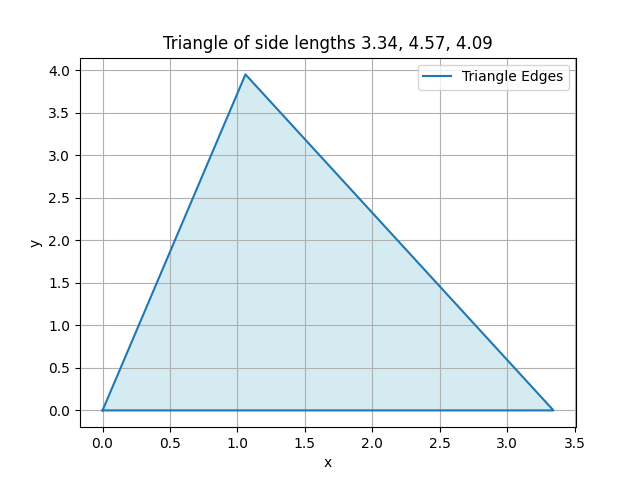
\includegraphics[width=0.8\textwidth]{figs/fig.png}
    \caption{Triangle Satisfying given conditions}
    \end{figure}   
%
%The radius  of $C$ is obtained as
%\begin{align}
%r = \norm{O-P} = 2
%\end{align}
\end{frame}
\end{document}

